% Options for packages loaded elsewhere
\PassOptionsToPackage{unicode}{hyperref}
\PassOptionsToPackage{hyphens}{url}
%
\documentclass[
  ignorenonframetext,
]{beamer}
\usepackage{pgfpages}
\setbeamertemplate{caption}[numbered]
\setbeamertemplate{caption label separator}{: }
\setbeamercolor{caption name}{fg=normal text.fg}
\beamertemplatenavigationsymbolsempty
% Prevent slide breaks in the middle of a paragraph
\widowpenalties 1 10000
\raggedbottom
\setbeamertemplate{part page}{
  \centering
  \begin{beamercolorbox}[sep=16pt,center]{part title}
    \usebeamerfont{part title}\insertpart\par
  \end{beamercolorbox}
}
\setbeamertemplate{section page}{
  \centering
  \begin{beamercolorbox}[sep=12pt,center]{part title}
    \usebeamerfont{section title}\insertsection\par
  \end{beamercolorbox}
}
\setbeamertemplate{subsection page}{
  \centering
  \begin{beamercolorbox}[sep=8pt,center]{part title}
    \usebeamerfont{subsection title}\insertsubsection\par
  \end{beamercolorbox}
}
\AtBeginPart{
  \frame{\partpage}
}
\AtBeginSection{
  \ifbibliography
  \else
    \frame{\sectionpage}
  \fi
}
\AtBeginSubsection{
  \frame{\subsectionpage}
}
\usepackage{amsmath,amssymb}
\usepackage{iftex}
\ifPDFTeX
  \usepackage[T1]{fontenc}
  \usepackage[utf8]{inputenc}
  \usepackage{textcomp} % provide euro and other symbols
\else % if luatex or xetex
  \usepackage{unicode-math} % this also loads fontspec
  \defaultfontfeatures{Scale=MatchLowercase}
  \defaultfontfeatures[\rmfamily]{Ligatures=TeX,Scale=1}
\fi
\usepackage{lmodern}
\ifPDFTeX\else
  % xetex/luatex font selection
\fi
% Use upquote if available, for straight quotes in verbatim environments
\IfFileExists{upquote.sty}{\usepackage{upquote}}{}
\IfFileExists{microtype.sty}{% use microtype if available
  \usepackage[]{microtype}
  \UseMicrotypeSet[protrusion]{basicmath} % disable protrusion for tt fonts
}{}
\makeatletter
\@ifundefined{KOMAClassName}{% if non-KOMA class
  \IfFileExists{parskip.sty}{%
    \usepackage{parskip}
  }{% else
    \setlength{\parindent}{0pt}
    \setlength{\parskip}{6pt plus 2pt minus 1pt}}
}{% if KOMA class
  \KOMAoptions{parskip=half}}
\makeatother
\usepackage{xcolor}
\newif\ifbibliography
\setlength{\emergencystretch}{3em} % prevent overfull lines
\providecommand{\tightlist}{%
  \setlength{\itemsep}{0pt}\setlength{\parskip}{0pt}}
\setcounter{secnumdepth}{-\maxdimen} % remove section numbering
\usepackage{../../beamer_style/beamer_style}
\ifLuaTeX
  \usepackage{selnolig}  % disable illegal ligatures
\fi
\usepackage{bookmark}
\IfFileExists{xurl.sty}{\usepackage{xurl}}{} % add URL line breaks if available
\urlstyle{same}
\hypersetup{
  pdftitle={Introduction \& Syllabus},
  pdfauthor={Jake S. Truscott, Ph.D},
  hidelinks,
  pdfcreator={LaTeX via pandoc}}

\title{Introduction \& Syllabus}
\subtitle{POS6933: Computational Social Science}
\author{Jake S. Truscott, Ph.D}
\date{}
\institute{\vspace{-5mm}

University of Florida \newline Spring 2026 \newline \newline \newline

\includegraphics[width=3cm]{../../beamer_style/UF.png} \quad 

\includegraphics[width=3.1cm]{../../images/CSS_POLS_UF_Logo.png}}

\begin{document}
\frame{\titlepage}

\begin{frame}{Overview}
\phantomsection\label{overview}
\begin{itemize}
\item
  Course Introduction \& Overview

  \par \vspace{2.5mm}
\item
  Readings, Grading, Evaluation, and Expectations

  \par \vspace{2.5mm}
\item
  Introductions (Get to Know You!)

  \par \vspace{2.5mm}
\item
  Break!

  \par \vspace{2.5mm}
\item
  Downloading \texttt{R} and \texttt{Python}

  \par \vspace{2.5mm}
\item
  File (Data) Storage \& Management

  \par \vspace{2.5mm}
\item
  Reproducibility

  \par \vspace{2.5mm}
\end{itemize}
\end{frame}

\section{Course Overview}\label{course-overview}

\begin{frame}{Computational Social Science}
\phantomsection\label{computational-social-science}
\begin{itemize}
\tightlist
\item
  Computational Social Science is an incredibly broad sub-field within
  scope of political science. Particularly useful for concepts including
  (but not limited to):

  \par \vspace{2.5mm}

  \begin{itemize}
  \tightlist
  \item
    \footnotesize \textbf{Text as Data}: Analyses of legislative
    speeches, party platforms, and court opinions to measure ideology,
    framing, and rhetorical strategies.
  \item
    \footnotesize \textbf{Social Media \& Online Behavior}: Mined to
    study political communication, polarization, misinformation, and
    mobilization.
  \item
    \footnotesize \textbf{Networks \& Relationships}: Mapping
    legislative coalitions, donor connections, and influence in lobbying
    or policymaking.
  \item
    \footnotesize \textbf{Simulation \& Modeling}: Agent-based and
    computational models simulate collective action, polarization, and
    institutional processes.
  \item
    \footnotesize \textbf{Elections \& Campaigns}: Modeling to help
    forecast elections.
  \end{itemize}
\end{itemize}
\end{frame}

\begin{frame}{Computational Social Science (Cont.)}
\phantomsection\label{computational-social-science-cont.}
\begin{itemize}
\tightlist
\item
  We don't have time to cover every layer of methodology or substantive
  concept (\emph{nor would I feel qualified}\ldots)
\item
  Instead, we are largely going to focus on two goals for this semester:

  \par \vspace{2.5mm}
  \begin{enumerate}
  \item Improve your proficiency and competency with programming in \texttt{R} and (to a lesser extent) \texttt{Python} \par \vspace{2.5mm}
  \item Introduce methodologies primarily in the realm of \texttt{Text as Data} – with an eye towards both conceptual knowledge and application.
  \end{enumerate}
\end{itemize}
\end{frame}

\begin{frame}{Computational Social Science (Cont.)}
\phantomsection\label{computational-social-science-cont.-1}
\begin{itemize}
\tightlist
\item
  By the end of the semester, you should be able to:

  \par \vspace{2.5mm}

  \begin{itemize}
  \tightlist
  \item
    Conduct advanced computing routines, including multi-layered and
    hierarchical coding structures \footnotesize (e.g., iterative loops,
    data organization and manipulation, functions, package construction,
    etc.)

    \par \vspace{1.5mm}
  \item
    Retrieve, process, and organize non-traditional data sources (e.g.,
    text) for classification tasks using a combination of natural
    language processes (e.g., supervised, unsupervised, and
    self-supervised learning models)

    \par \vspace{1.5mm}
  \item
    Create informative representations of data and other summary
    findings (e.g., tables and figures)

    \par \vspace{1.5mm}
  \item
    Produce replicable coding routines using compilation suites in R,
    Python, and LaTex(Beamer)

    \par \vspace{1.5mm}
  \end{itemize}
\end{itemize}
\end{frame}

\section{Materials and Evaluation}\label{materials-and-evaluation}

\begin{frame}{Materials and Evaluation -- Textbooks and Readings}
\phantomsection\label{materials-and-evaluation-textbooks-and-readings}
\begin{columns}[T] % top-aligned columns
  \begin{column}{0.65\textwidth}
  \par \vspace{2.5mm}
  
  \begin{itemize}
  
  \item  \textbf{Required}: Grimmer, J., Roberts, M. E., \& Stewart, B. M. (2022). \emph{Text as data: A new framework for machine learning and the social sciences}. Princeton University Press. \par \vspace{2.5mm}
  
  \item \textbf{Recommended}: Llaudet, E., \& Imai, K. (2023). \emph{Data analysis for social science: A friendly and practical introduction}. Princeton University Press. \par \vspace{2.5mm}
  
  \item Articles Posted to Canvas (Have all readings complete before coming to class!)
  
  \end{itemize}
  \end{column}

  \begin{column}{0.35\textwidth}
    \centering
    
\includegraphics[width=0.55\linewidth]{../../images/text_as_data.jpg} \par \vspace{1mm}
    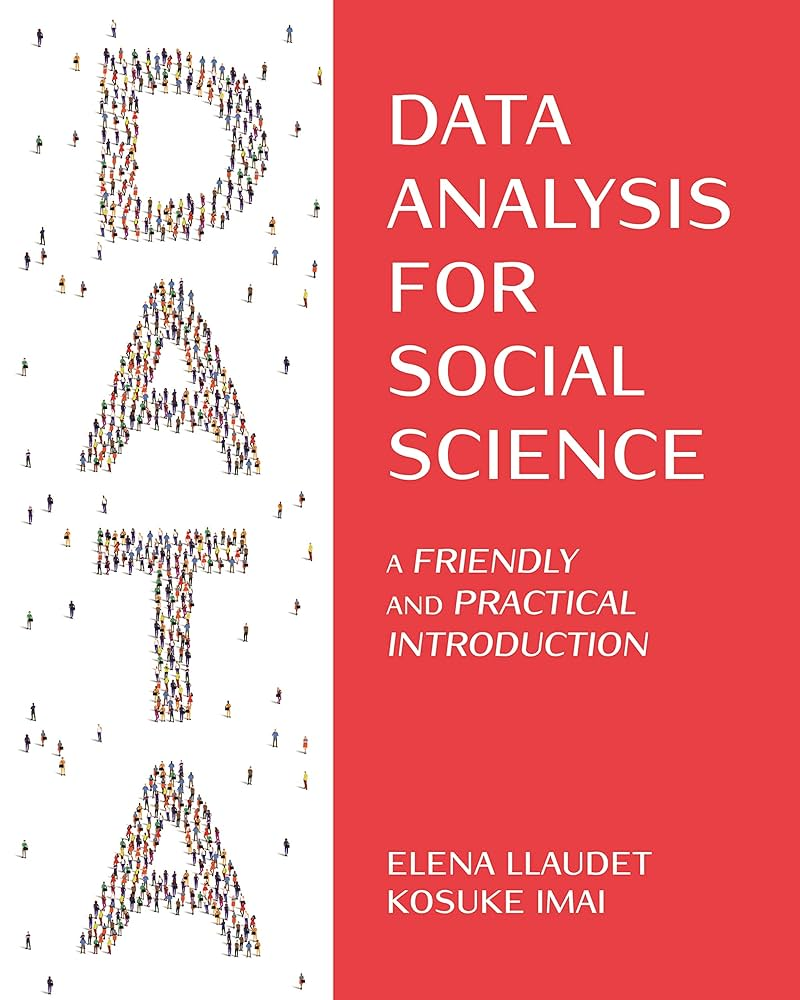
\includegraphics[width=0.55\linewidth]{../../images/data_analysis_for_social_science.jpg}

  \end{column}
\end{columns}
\end{frame}

\begin{frame}{Materials and Evaluation -- Grading \& Evaluation}
\phantomsection\label{materials-and-evaluation-grading-evaluation}
Weekly Problem Sets \dotfill 40\%

\par \vspace{1.5mm}

Participation \dotfill 10\%

\par \vspace{1.5mm}

Final Project \& Presentation \dotfill 50\%

\par \vspace{1.5mm}
\end{frame}

\begin{frame}{Materials and Evaluation -- Evaluation (Problem Sets)}
\phantomsection\label{materials-and-evaluation-evaluation-problem-sets}
\begin{itemize}
\tightlist
\item
  Problem sets due to Canvas on Sundays by 11:59pm

  \par \vspace{1.5mm}
\item
  I will drop the two submissions with lowest marks

  \par \vspace{1.5mm}
\item
  Must be compiled using \texttt{RMarkdown} -- We will discuss file
  organization today

  \par \vspace{1.5mm}
\item
  We will spend the first 30min-1hr of each class period reviewing the
  problem set from the week before.
\end{itemize}
\end{frame}

\begin{frame}{Materials and Evaluation -- Expectations}
\phantomsection\label{materials-and-evaluation-expectations}
Expectations are fairly simple:

\par \vspace{5mm}

\begin{enumerate}

\item Come to Class Prepared \& Ready to Learn  \par \vspace{2.5mm}

\item Don't Be Afraid to Ask for Help  \par \vspace{2.5mm}

\item Embrace the Learning Curve


\end{enumerate}
\end{frame}

\begin{frame}{Materials and Evaluation -- Other Notes}
\phantomsection\label{materials-and-evaluation-other-notes}
\begin{itemize}
\tightlist
\item
  The course is technology driven -- You need to come prepared with a
  laptop capable of downloading \texttt{R}, \texttt{RStudio}, and
  \texttt{Python}

  \par \vspace{2.5mm}
\item
  I am maintaining a GitHub Repository and website for the course:
  \url{https://jaketruscott.github.io/CSS_POS_UF/}

  \par \vspace{2.5mm}
\item
  The website has many additional resources for each week of the
  semester.
\end{itemize}
\end{frame}

\section{Introductions}\label{introductions}

\begin{frame}{About Me -- Jake S. Truscott, Ph.D.}
\phantomsection\label{about-me-jake-s.-truscott-ph.d.}
\begin{columns}[T] % top-aligned columns
  \begin{column}{0.65\textwidth}
  \par \vspace{2.5mm}
  
  \begin{itemize}
  
  \item Research Focus: American Judiciary \& CSS  \par \vspace{2.5mm}
    \item Proud UGA Grad \par \vspace{1.5mm}
    \item Fav Conspiracy Theory: The New York Mets are a Though Experiment Created by Harvard University to Study the Emotional Pain Tolerance of American Sports Fans \par \vspace{1.5mm}
    \item My Wife is Very Pregnant -- We may need to skip a week last minute in late-February/early-March (TBD) \par \vspace{1.5mm}
  \end{itemize}
  \end{column}

  \begin{column}{0.5\textwidth}
    \centering
    \vspace{2.5mm}
    
\includegraphics[width=0.75\linewidth]{../../images/me.jpg}
    \vfill

  \end{column}
\end{columns}
\end{frame}

\begin{frame}{About You}
\phantomsection\label{about-you}
\begin{itemize}
\tightlist
\item
  Name

  \par \vspace{2.5mm}
\item
  Research Focus

  \par \vspace{2.5mm}
\item
  Fun Fact or Hot Take

  \par \vspace{2.5mm}
\end{itemize}
\end{frame}

\section{Break}\label{break}

\section{\texorpdfstring{Downloading
\texttt{R}}{Downloading }}\label{downloading}

\begin{frame}{Downloading \texttt{R}}
\phantomsection\label{downloading-1}
\begin{columns}[T] % top-aligned columns
  \begin{column}{0.65\textwidth}
  \par \vspace{2.5mm}
  \begin{itemize}
  
  \item \texttt{R} is a programming language and environment for statistical computing and data analysis. \par \vspace{2.5mm}
  
  \item It is designed specifically for working with data, running statistical tests, creating models, and visualizing results. \par \vspace{2.5mm}
  
  \item \textbf{Why \texttt{R} and not \texttt{Stata} or \texttt{Python}} (exclusively)? \par \vspace{2.5mm}
  
  \item \texttt{R} is incredibly flexible, more intuitive, easily accessible, and free! 
  
  \end{itemize}
  \end{column}

  \begin{column}{0.5\textwidth}
    \centering
    \vspace{2.5mm}
    
\includegraphics[width=0.75\linewidth]{../../images/R_logo.png}
    \vfill

  \end{column}
\end{columns}
\end{frame}

\begin{frame}{Downloading \texttt{R} (Cont.)}
\phantomsection\label{downloading-cont.}
\begin{itemize}
\tightlist
\item
  We will use \texttt{R} for just about everything in this course.

  \par \vspace{1.5mm}
\item
  Even when we shift to tools better suited for \texttt{Python}, I will
  show you how can implement through \texttt{R}

  \par \vspace{1.5mm}
\item
  To download \texttt{R} and its companion IDE \texttt{RStudio}, visit:
  \url{https://jaketruscott.github.io/CSS_POS_UF/class_1/downloading_R.html}

  \par \vspace{1.5mm}
\end{itemize}
\end{frame}

\section{\texorpdfstring{Downloading
\texttt{Python}}{Downloading }}\label{downloading-2}

\begin{frame}{Downloading \texttt{Python}}
\phantomsection\label{downloading-3}
\begin{columns}[T] % top-aligned columns
  \begin{column}{0.65\textwidth}
  \par \vspace{2.5mm}
  \begin{itemize}
  
  \item \texttt{Python} is a versatile, general-purpose programming language – it can be used for web development, data analysis, automation, machine learning, and more. \par \vspace{1.5mm}
  
  \item Many of you may already have exposure to \texttt{Python} from Dr. Arfi's classes -- You are welcome to use more \texttt{Python} if you so choose, though I will be teaching \texttt{R} primarily.  \par \vspace{1.5mm}
  
  \item To download \texttt{R} and its companion IDE \texttt{RStudio}, visit: \url{https://jaketruscott.github.io/CSS_POS_UF/class_1/downloading_Python.html} \par \vspace{1.5mm}

  
  \end{itemize}
  \end{column}

  \begin{column}{0.5\textwidth}
    \centering
    \vspace{2.5mm}
    
\includegraphics[width=0.75\linewidth]{../../images/Python_logo.png}
    \vfill

  \end{column}
\end{columns}
\end{frame}

\section{Data Storage and
Organization}\label{data-storage-and-organization}

\end{document}
